\section{Thames Catchment Model (model ID: 25)}
The Thames Catchment Model (TCM) model (fig.~\ref{fig:25_schematic}) is originally intended to be used in zones with similar surface characteristics, rather than catchments as a whole \citep{Moore2001}. It has 4 stores and 6 parameters ($\phi$, $rc$, $\gamma$, $k_1$, $c_a$ and $k_2$). The model aims to represent:

\begin{itemizecompact}
\item Effective rainfall before infiltration;
\item Preferential recharge;
\item Catchment drying through prolonged soil moisture depletion;
\item Groundwater abstraction;
\item Non-linear groundwater flow.
\end{itemizecompact}

\subsection{MARRMoT model name}
m\_25\_tcm\_6p\_4s \\

% Equations
\subsection{Model equations}

% Model layout figure
{ 																	% This ensures it doesn't warp text further down
\begin{wrapfigure}{l}{5cm}
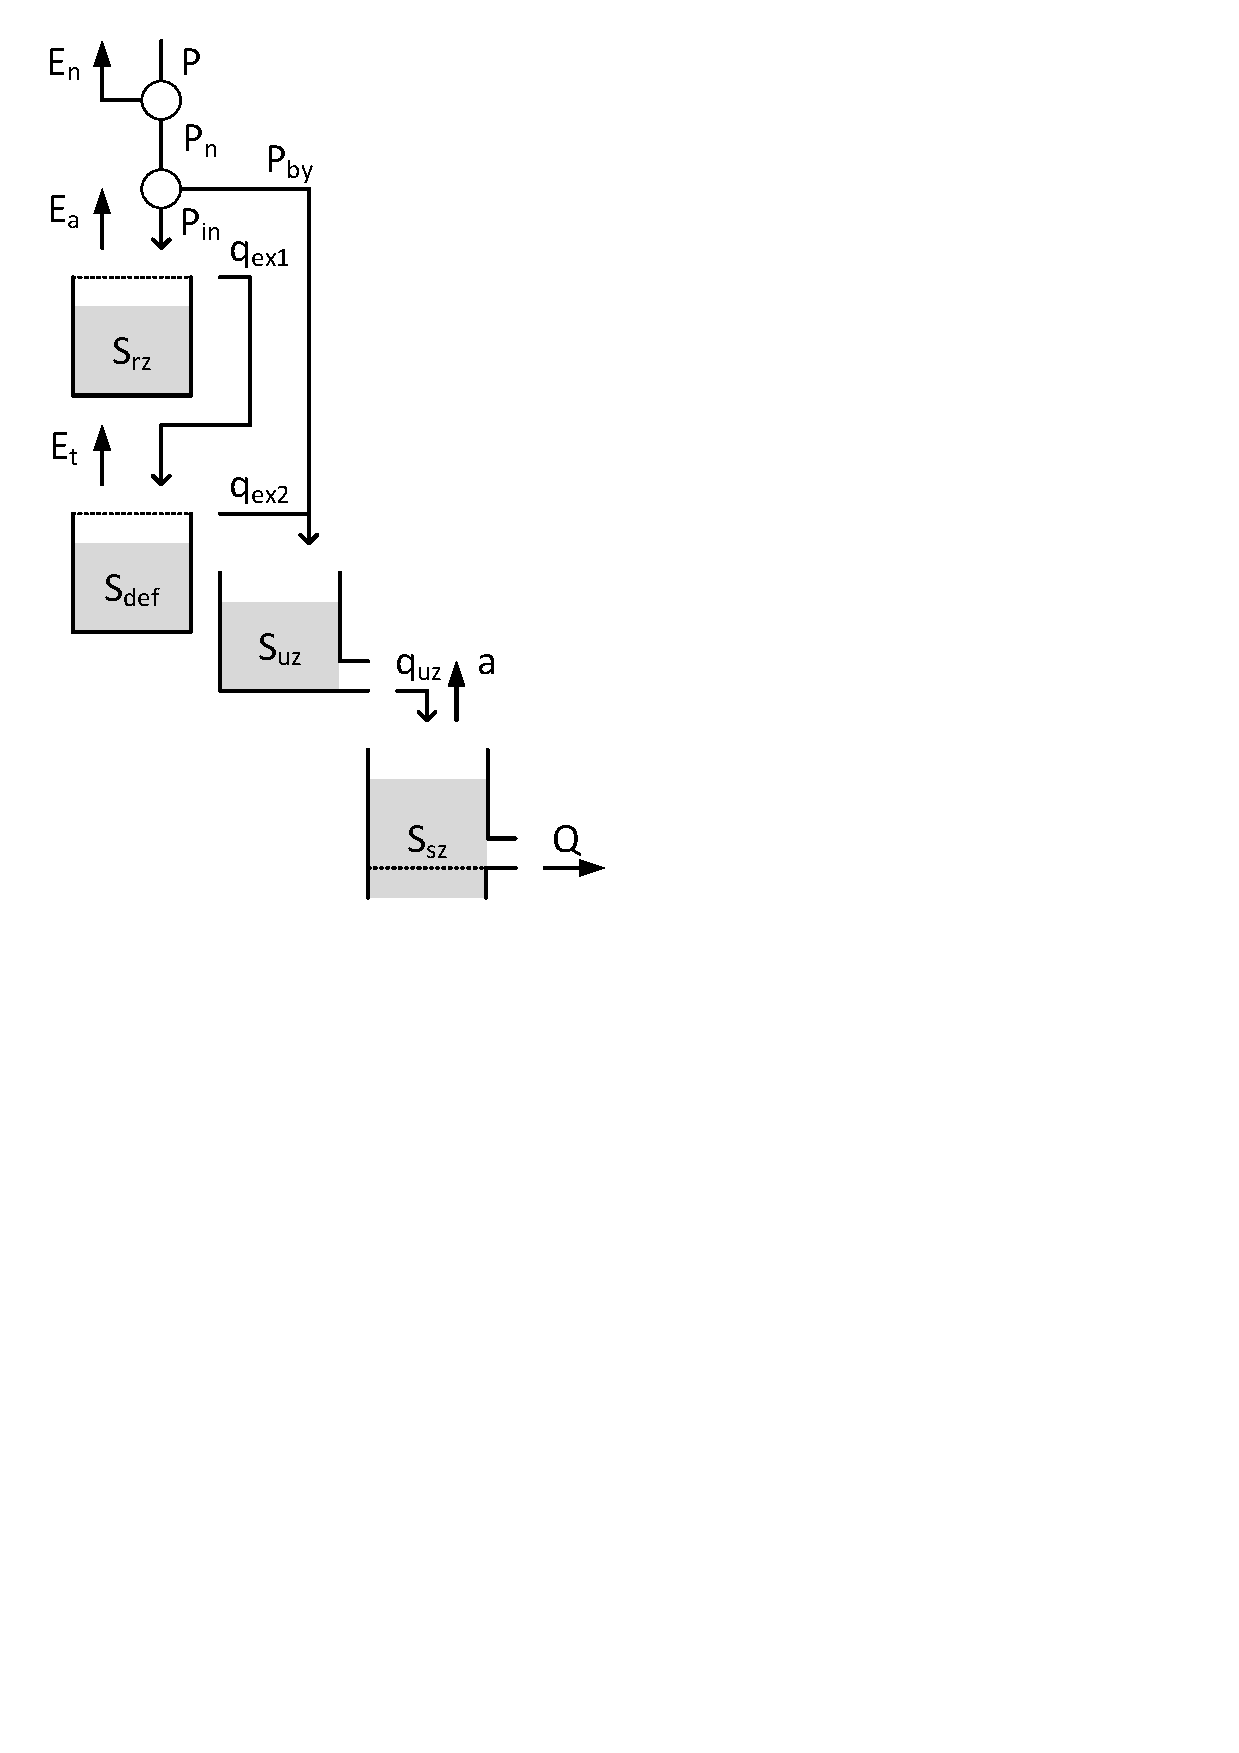
\includegraphics[trim=1cm 14.5cm 7cm 1cm,width=7cm,keepaspectratio]{./AppA_files/25_schematic.pdf}
\caption{Structure of the TCM model} \label{fig:25_schematic}
\end{wrapfigure}

\begin{align}
	\frac{dS_{Rz}}{dt} &= P_{in}-E_a-q_{ex1} \\
	P_{in} &= (1-\phi)*P_n \\
	P_n &= max(P-E_p,0)\\
	E_a &= 
	\begin{cases}
		E_p, & \text{if } S_{rz} > 0 \\
		0, & \text{otherwise}
	\end{cases}\\
	q_{ex1} &= \begin{cases}
		P_{in}, &\text{if } S_{rz} > rc \\
		0, & \text{otherwise} \\
	\end{cases} 
\end{align}

Where $S_{rz}$ [mm] is the current storage in the root zone, refilled by infiltrated precipitation $P_{in}$ $[mm/d]$, and drained by evaporation $E_a$ $[mm/d]$ and storage excess flow $q_{ex1}$ $[mm/d]$. 
$P_{in}$ is the fraction $(1-\phi)$ [-] of net precipitation $P_n$ $[mm/d]$ that is not preferential recharge. 
$P_n$ is the difference between precipitation $P$ [mm/d] and potential evapotranspiration $E_p$ [mm/d] per time step. 
$E_a$ occurs at the net potential rate whenever possible.
$q_{ex1}$ occurs only when the store is at maximum capacity $rc$ [mm].

} % end of wrapfigure fix

\begin{align}
	\frac{dS_{def}}{dt} &= E_t + q_{ex2} - q_{ex1}\\
	E_t &=\begin{cases}
		\gamma*E_p, &\text{if } S_{rz} = 0 \\
		0, & \text{otherwise} \\
	\end{cases} \\
	 q_{ex2}  &= \begin{cases}
		q_{ex1}, &\text{if } S_{def} = 0 \\
		0, & \text{otherwise} \\
	\end{cases}
\end{align}

Where $S_{def}$ [mm] is the current storage in the soil moisture \emph{deficit} store.
The deficit is increased by evaporation $E_t$ $[mm/d]$ and percolation $q_{ex2}$ $[mm/d]$.
The deficit is decreased by overflow from the upper store $q_{ex1}$.
$E_t$ only occurs when the upper zone is empty and at a fraction $\gamma$ [-] of $E_p$.
$q_{ex2}$ only occurs when the deficit is zero.

\begin{align}
	\frac{dS_{uz}}{dt} &= P_{by} + q_{ex2} - q_{uz} \\
	P_{by} &= \phi*P_n\\
	q_{uz} &= k_1*S_{uz}
\end{align}
  
Where $S_{uz}$ is the current storage in the unsaturated zone, refilled by preferential recharge $P_{by}$ $[mm/d]$ and percolation $q_{ex2}$ $[mm/d]$, and drained by groundwater flow $q_{uz}$ $[mm/d]$.
$P_{by}$ is a fraction $\phi$ [-] of $P_n$.
$q_{uz}$ has a linear relation with storage through time parameter $k_1$ $[d^{-1}]$.

\begin{align}
	\frac{dS_{sz}}{dt} &= q_{uz} -a-Q\\
	a &= c_a\\
	Q &= \begin{cases}
		k_2*S_{sz}^2, &\text{if } S_{sz} > 0 \\
		0, & \text{otherwise} \\
	\end{cases}
\end{align}

Where $S_{sz}$ [mm] is the current storage in the saturated zone, refilled by groundwater flow $q_{uz}$ $[mm/d]$ and drained by abstractions $a$ $[mm/d]$ and outflow $Q$ $[mm/d]$.
$a$ occurs at a constant rate $c_a$ $[mm/d]$.
Abstractions can draw down the aquifer below the runoff generating threshold. 
$Q$ has a quadratic relation with storage through parameter $k_2$ $[mm^{-1} d^{-1}]$.

\newpage
\subsection{Parameter overview}
% Table generated by Excel2LaTeX from sheet 'Sheet1'
\begin{table}[htbp]
  \centering
    \begin{tabular}{lll}
    \toprule
    Parameter & Unit  & Description \\
    \midrule
    $\phi$ & $-$   & Fraction of net precipitation that is preferntial flow \\
    $rc$  & $mm$  & Maximum root zone storage \\
    $\gamma$ & $-$   & Transpiration reduction factor \\
    $k_1$ & $d^{-1}$ & Runoff coefficient \\
    $c_a$ & $mm~d^{-1}$ & Abstraction rate \\
    $k_2$ & $d^{-1}$ & Runoff coefficient \\
    \bottomrule
    \end{tabular}%
  \label{tab:addlabel}%
\end{table}%

